              
                %%%%%%%%%%%%%%%%%%%%%%%%%%%%%%%%%%%%%%%%%%%%%%%%%%%%%%%%%%%%%%%%%%%%%%
% LaTeX Example: Project Report
%
% Source: http://www.howtotex.com
%
% Feel free to distribute this example, but please keep the referral
% to howtotex.com
% Date: March 2011 
% 
%%%%%%%%%%%%%%%%%%%%%%%%%%%%%%%%%%%%%%%%%%%%%%%%%%%%%%%%%%%%%%%%%%%%%%
% How to use writeLaTeX: 
%
% You edit the source code here on the left, and the preview on the
% right shows you the result within a few seconds.
%
% Bookmark this page and share the URL with your co-authors. They can
% edit at the same time!
%
% You can upload figures, bibliographies, custom classes and
% styles using the files menu.
%
% If you're new to LaTeX, the wikibook is a great place to start:
% http://en.wikibooks.org/wiki/LaTeX
%
%%%%%%%%%%%%%%%%%%%%%%%%%%%%%%%%%%%%%%%%%%%%%%%%%%%%%%%%%%%%%%%%%%%%%%
% Edit the title below to update the display in My Documents
%\title{Project Report}
%
%%% Preamble
\documentclass[paper=letter, fontsize=11pt]{scrartcl}
\usepackage{url}
\usepackage{color}
\usepackage{fourier}
\usepackage{listings}
\usepackage[T1]{fontenc}
\usepackage[spanish]{babel}
\selectlanguage{spanish}
\usepackage{hyperref}
\usepackage[pdftex]{graphicx}
\usepackage[margin=2.5cm]{geometry}
\usepackage{amsmath,amsfonts,amsthm} % Math packages
                                       % English language/hyphenation
\usepackage[protrusion=true,expansion=true]{microtype}  

%%% Maketitle metadata
\newcommand{\horrule}[1]{\rule{\linewidth}{#1}}     % Horizontal rule

\title{
        %\vspace{-1in}  
        \usefont{OT1}{bch}{b}{n}
        \normalfont \normalsize \textsc{Universidad de los Andes, Departamento de F\'isica \\
        F\'isica at\'omica} \\ [25pt]
        \horrule{0.5pt} \\[0.4cm]
        \huge Valores esperados \\
        \horrule{2pt} \\[0.5cm]
}
\author{
        \normalfont                                 \normalsize
        Juan Barbosa, 201325901\\[-3pt]      \normalsize
        Marzo 23, 2017
}
\date{}

\lstset{keywordstyle=\color{blue}, basicstyle=\scriptsize, frame=single, language=Python}

%%% Begin document
\begin{document}
\maketitle

\[
\boxed{-\dfrac{\hbar^2}{2m}\nabla^2\Psi(x) + V(x)\Psi(x) = E\Psi(x)}
\]

Para el \'atomo de hidr\'ogeno la ecuaci\'on anterior se escribe usando coordenedas esf\'ericas, cuyo potencial depende de la parte radial:
\begin{equation}
	V(r) = \dfrac{ze^2}{4\pi\epsilon_0r}
\end{equation}

Haciendo un cambio de variable $r=\dfrac{a_0}{z}u$ se puede reescribir la ecuaci\'on para la parte radial como:
\begin{equation}
	\dfrac{d^2R}{du^2} + \dfrac{2}{u}\dfrac{dR}{du} + \left(\epsilon - \dfrac{2}{u} - \dfrac{l(l+1)}{u^2}\right)R = 0
	\qquad \text{donde } \epsilon=\dfrac{E}{E_0}
\end{equation}

Para obtener el valor esperado de $r$ se usa la probabilidad radial $P=4\pi R^2r^2/\int Pdr$.
\begin{equation}
	<r> = <a_0u> = a_0<u> = a_0\int\limits_{0}^{30}Pudu
\end{equation}

El valor esperado de $<\Delta E>$ se calcula de la siguiente manera:
\begin{equation}
	<\Delta E> = \dfrac{\hbar^2}{4m^2c^2}<1/rdV/dr>\left[j(j+1)-l(l+1)-s(s+1)\right] = \alpha <1/rdV/dr> \beta
\end{equation}

donde $\alpha$ corresponde con una constante y $\beta$ depende de $j, l, s$. Tomando la derivada de la ecuaci\'on 1 y diviendo por r. se obtiene.
\begin{equation}
	<\Delta E> = \alpha \dfrac{e^2}{4\pi\epsilon_0}<1/r^3>\beta = \alpha \dfrac{e^2}{4\pi\epsilon_0a_0^3}<1/u^3>\beta
\end{equation}

Teniendo en cuenta $u$ y $\beta$ son adimensionales las unidades est\'an dadas por $\alpha\frac{e^2}{4\pi\epsilon_0a_0^3}$ cuyo valor es $3.62\times 10^{-4}$ eV. Para finalmente obtener:
\begin{equation}
	<\Delta E> = 3.62\beta\times 10^{-4}\int\limits_{0}^{30}Pu^{-3}du
\end{equation}

Para $\beta$, $j = l\pm s$ siempre que $l>0$, de lo contrario $j = s$, donde $s=1/2$.
\lstinputlisting{finder.py}

\begin{figure}[!ht]
	\centering
	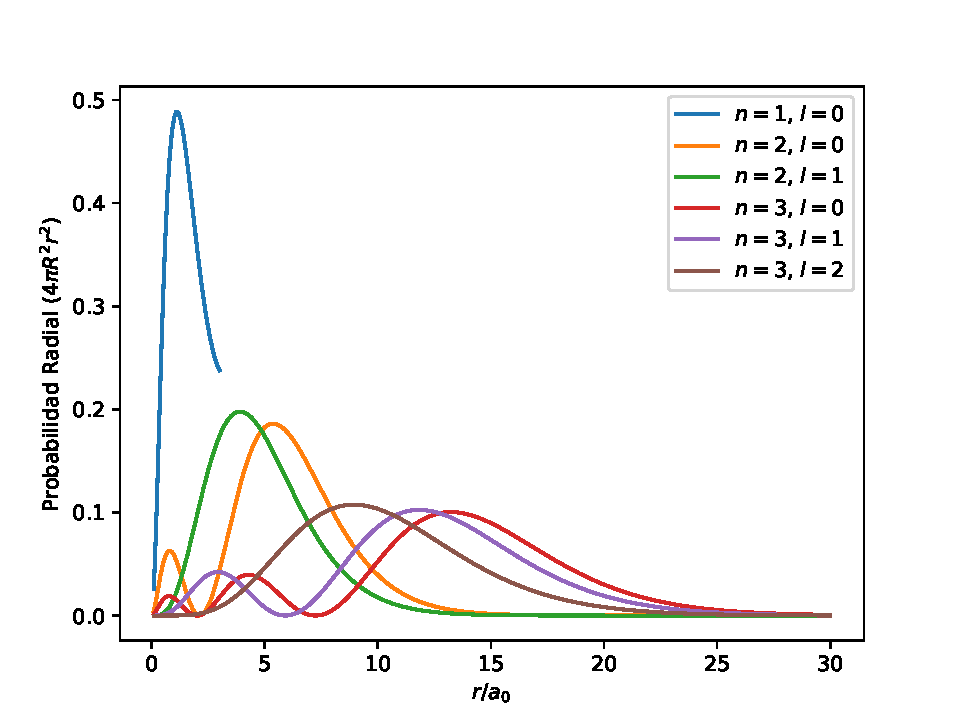
\includegraphics[width=\linewidth]{probability.pdf}
	\caption{Funci\'on normalizada de probabilidad. Para distintos valores de $n$ y $l$.}
	\label{fig:prop}
\end{figure}

La \autoref{fig:prop} muestra el comportamiento de la probabilidad radial en funci\'on del radio. En ella se puede observar que para un mismo valor de $n$, el m\'aximo de las funciones se ubica a menor radio conforme $l$ aumenta, \autoref{fig:functions}. Lo anterior tambi\'en se evidencia en la \autoref{tb: table} donde se expone el valor esperado para $r$, el cual disminuye conforme $l$ aumenta en un mismo nivel de energ\'ia. Adicionalmente el valor esperado se encuentra a valores m\'as altos de $r$ que el m\'aximo de la distribuci\'on.

Respecto a los valores esperados para $\Delta E$ se observa que dependiendo del valor de $j$ la eneg\'ia aumenta o disminuye, sin embargo no lo hacen en la misma proporci\'on. Para todos los casos la disminuci\'on es mayor al aumento por lo cual es acoplamiento sp\'in \'orbita contribuye a la estabilidad del \'atomo.

Finalmente y a pesar que existen pocos puntos, es posible determinar que el valor esperado de $r$ var\'ia con $n^2$, con pendiente constante con valor $a_0$, resultado obtenido por Bohr.
\begin{equation}
	r = a_0n^2
\end{equation}

\begin{table}[h]
	\centering
	\caption{Valores esperados para $r$ y $\Delta E$. $E_1$ corresponde con $j=l+s$ y $E_2$ con $j=l-s$.}
	\begin{tabular}{ccccc}
		\hline
		$n$ & $l$ & $<r>/a_0$ & $\Delta E_1$ (eV) & $\Delta E_2$ eV \\
		\hline
		1 & 0 & 1.539 & 0.000e+00 & -1.141e-03 \\
		2 & 0 & 6.070 & 0.000e+00 & -1.932e-04 \\
		2 & 1 & 4.911 & 1.631e-05 & -3.261e-05 \\
		3 & 0 & 13.543 & 0.000e+00 & -5.971e-05 \\
		3 & 1 & 12.272 & 5.021e-06 & -1.004e-05 \\
		3 & 2 & 10.439 & 1.820e-06 & -2.730e-06 \\
		\hline
	\end{tabular}
	\label{tb: table}
\end{table}

\begin{figure}[ht]
	\centering
	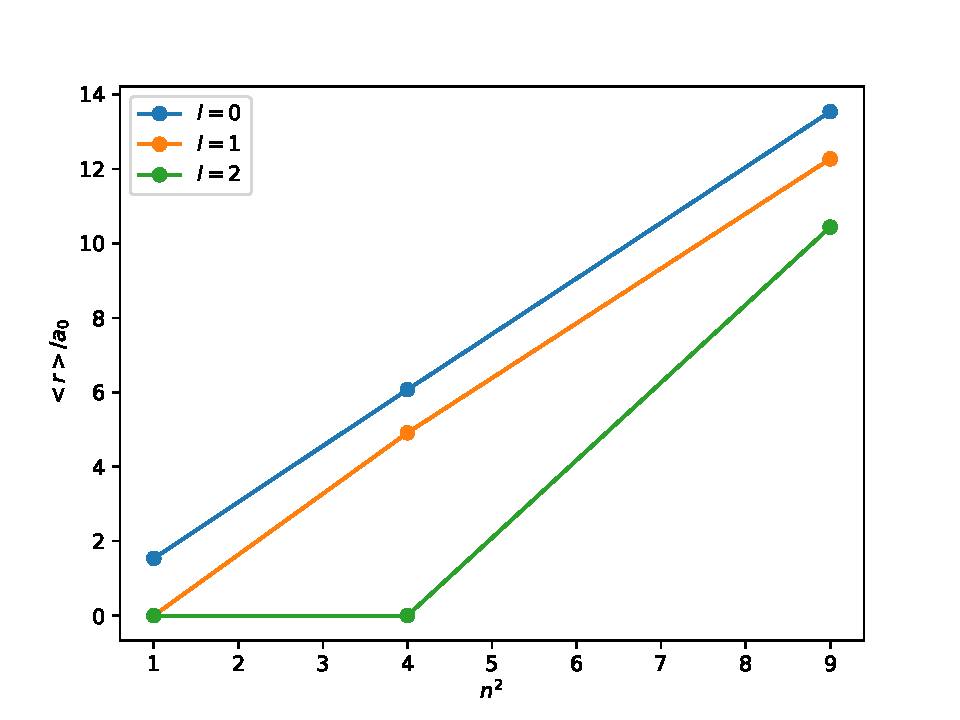
\includegraphics[width=\linewidth]{radius.pdf}
	\caption{Valor esperado de $r$ en funci\'on de $n$ para distintos valores de $l$.}
	\label{fig:functions}
\end{figure}
\end{document}
              